\section{Generacja kodu pośredniego}
	
	Kod pośredni -- jest to język, składający się z elementarnych operacji nad danymi, takimi jak
	arytmetyczne operacje, zapisanie do komórki pamięci.
	\\
	
	Im prostszy ten język jest, tym prostsze
	są algorytmy do analizy, optymalizacji i generacji dalszych warstw pośrednich.
	\\
	
	Istnieje wiele różnych podobnych do assemblera języków (Intermediate representation, \textbf{IR}), służących
	do generacji kodu maszynowego (LLVM IR, GIMPLE, FIRM). Każdy z nich jest doskonale zaprojektowany, dopasowany
	do wielu języków programowania. Naprzykład, LLVM IR jest użyty jako backend w Clang, Glasgow Haskell Compiler,
	w językach Rust, Swift i innych. Biorąc gotową warstwę IR, pozbawiamy się wysiłku na zaprojektowanie samego
	języka, SSA, optymalizacji. Aby zrobić to, wymagana jest grupa ekspertów i kilka lat ciężkiej pracy.
	\\

	Niniejszy IR jest tylko i wyłącznie edukacyjny, mający na celu pokazanie ogólnego kształtu warstw pośrednich.
	Oczywiście, podmiana własnego IR na inny skali produkcyjnej da nieograniczone możliwości i mocno popchnie
	rozwoj języka do przodu.

	\subsection{Algorytm}
		Generator IR przyjmuje AST jako wejście. Stworzenie instrukcji pośrednich
		polega na rekurencyjnym przejściu tego drzewa oraz tłumaczeniu danych o
		programie z poziomu drzewa (w zasadzie elementów syntaksycznych) na język
		niskiego poziomu. W zależności od węzła musi być stworzony kod, zachowujący
		się zgodnie z oczekiwaniem użytkownika.
		\\
		
		Naprzykład, pętla while (po lewej stronie) zostanie przetłumaczona na
		kod niskiego poziomu (po prawej stronie).

		\begin{center}
		\begin{tabular}{ c c c }
\begin{lstlisting}[label={lst:warn-unused-var},linewidth=6.5cm]
int main() {
    int i = 1;
    while (i < 10 && i != 0)
    {
        int j = i;
        ++j;
        ++i;
    }
    return 0;
}			
.
.
.
.
.
.
.
\end{lstlisting}
		& &	
\begin{lstlisting}[label={lst:warn-unused-var},linewidth=8cm]
fun main():
       0:   int t0
       1:   t0 = 1
       2:   | int t1
       3:   | int t2
       4:   | t2 = t0 < 10
       5:   | int t3
       6:   | t3 = t0 != 0
       7:   | t1 = t2 && t3
       8:   | if t1 != 0 goto L10
       9:   | jmp L15
      10:   | int t4
      11:   | t4 = t0
      12:   | t4 = t4 + 1
      13:   | t0 = t0 + 1
      14:   | jmp L2
      15:   ret 0
\end{lstlisting}
		\end{tabular}
		\end{center}
		
		Widać, że złożona semantycznie konstrukcja \texttt{while} została
		przedstawiona za pomocą prostszych do wykonania operacji: stworzyć
		zmienną o rozmiarze N bajtów, zapisać do niej wynik operacji binarnej,
		wykonać skok do instrukcji o pewnym indeksie. Analogicznie przedstawione są
		inne części języka (\texttt{for}, \texttt{do while}, \texttt{if}). Oczywiście,
		wszystkie konstrukcje mogą być zagnieżdżone dowolną ilośc razy, przy tym
		zachowawszy liniową strukturę IR.

	\subsection{Instrukcje}

	Zdefiniowane w implementacji struktury dzielą się
	na instrukcje i typy danych.

	\begin{center}
		\setlength{\tabcolsep}{0.5em}
		\renewcommand{\arraystretch}{1.5}
		\definecolor{instrc}{gray}{0.4}
		\begin{tabular}{| L{0.2\linewidth} | L{0.75\linewidth} | }
			\hline
			\textbf{Instrukcja} & \textbf{Opis} \\
			\hline
			\textcolor{instrc}{\textbf{ir\_alloca}}
				& Alokacja określonej ilości bajtów
                 na stosie. \\
			\hline
			\textcolor{instrc}{\textbf{ir\_alloca\_array}}
            	& Alokacja określonej ilości bajtów
				  na stosie, pomnożonej przez rozmiar
                  tablicy. \\
			\hline
			\textcolor{instrc}{\textbf{ir\_store}} 
				& Zapisanie wartości do zmiennej
                  lub do tablicy o wskazanym
                  indeksie. \\
			\hline

			\textcolor{instrc}{\textbf{ir\_jump}}
				& Przekazanie przepływu sterowania
                  do instrukcji o wskazanym indeksie. \\
			\hline
			\textcolor{instrc}{\textbf{ir\_cond}}
				& Instrukcja warunkowa. Wykonuje skok
         	     (taki sam, jak \texttt{ir\_jump}),
                  jeżeli warunek jest spełniony.
                  Inaczej sterowanie się przekazuje
                  do następnej instrukcji. \\
			\hline
			\textcolor{instrc}{\textbf{ir\_ret}}
				& Wyjście z funkcji. Może mieć lub nie
                  mieć wartość zwracaną. \\
  			\hline
  			\textcolor{instrc}{\textbf{ir\_fn\_call}}
                & Wywołanie funkcji. \\
            \hline
		\end{tabular}
	\end{center}
	
	\spacing

	\begin{center}
		\setlength{\tabcolsep}{0.5em}
		\renewcommand{\arraystretch}{1.5}
		\definecolor{instrc}{gray}{0.4}
		\begin{tabular}{| L{0.2\linewidth} | L{0.75\linewidth} | }
			\hline
			\textbf{Typ} & \textbf{Opis} \\
			\hline
			\textcolor{instrc}{\textbf{ir\_imm}}
				& Wartość (int, char, bool). \\
            \hline
			\textcolor{instrc}{\textbf{ir\_string}}
				& Łańcuch znaków. \\
			\hline
			\textcolor{instrc}{\textbf{ir\_sym}}
				& Indeks zmiennej. \\
			\hline
			\textcolor{instrc}{\textbf{ir\_bin}}
				& Operacja binarna (dwuargumentowa). \\
			\hline
			\textcolor{instrc}{\textbf{ir\_member}}
				& Operacja dostępu do indeksu tablicy. \\
			\hline
			\textcolor{instrc}{\textbf{ir\_type\_decl}}
				& Definicja typu. \\
			\hline
			\textcolor{instrc}{\textbf{ir\_fn\_decl}}
				& Definicja funkcji. \\
			\hline
		\end{tabular}
	\end{center}

	\subsection{Generacja grafu sterowania}

	\tikzstyle{process} = [rectangle, minimum width=3cm, minimum height=0.5cm,text centered, draw=black]
	\tikzstyle{arrow} = [thick,->,>=stealth]

	\begin{center}
		\begin{tabularx}{\textwidth}{ L{9cm} L{9cm} }

		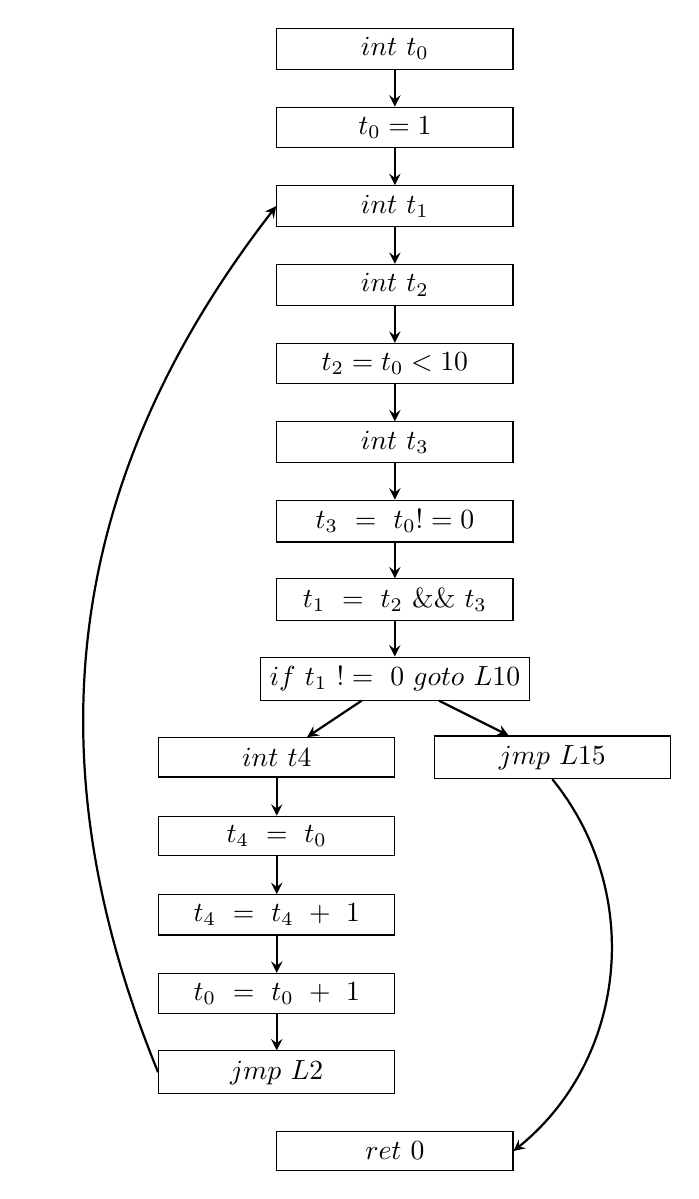
\begin{tikzpicture}[node distance=1cm]
			\node (0) [process] {$int \ t_0$};
			\node (1) [process, below of=0] {$t_0 = 1$};
			\node (2) [process, below of=1] {$int \ t_1$};
			\node (3) [process, below of=2] {$int \ t_2$};
			\node (4) [process, below of=3] {$t_2 = t_0 < 10$};
			\node (5) [process, below of=4] {$int \ t_3$};
			\node (6) [process, below of=5] {$t_3 \ = \ t_0 != 0$};
			\node (7) [process, below of=6] {$t_1 \ = \ t_2 \ \&\& \ t_3$};
			\node (8) [process, below of=7] {$if \ t_1 \ != \ 0 \ goto \ L10$};
			\node (9) [process, below of=8, right of=8, xshift=1cm] {$jmp \ L15$};
			\node (10) [process, below of=8, xshift=-1.5cm] {$int \ t4$};
			\node (11) [process, below of=10] {$t_4 \ = \ t_0$};
			\node (12) [process, below of=11] {$t_4 \ = \ t_4 \ + \ 1$};
			\node (13) [process, below of=12] {$t_0 \ = \ t_0 \ + \ 1$};
			\node (14) [process, below of=13] {$jmp \ L2$};
			\node (15) [process, below of=14, xshift=1.5cm] {$ret \ 0$};

			\draw [arrow] (0) -- (1);
			\draw [arrow] (1) -- (2);
			\draw [arrow] (2) -- (3);
			\draw [arrow] (3) -- (4);
			\draw [arrow] (4) -- (5);
			\draw [arrow] (5) -- (6);
			\draw [arrow] (6) -- (7);
			\draw [arrow] (7) -- (8);
			\draw [arrow] (8) -- (9);
			\draw [arrow] (8) -- (10);
			\draw [arrow, bend left=45] (9.south) to (15.east);
			\draw [arrow] (10) -- (11);
			\draw [arrow] (11) -- (12);
			\draw [arrow] (12) -- (13);
			\draw [arrow] (13) -- (14);
			\draw [arrow, bend left=30] (14.west) to (2.west);
		\end{tikzpicture}
	&
	Wygenerowana poprzednio warstwa poprzednia zawiera wszystkie informacje, dotyczące operacji nad
	danymi, ale brakuje jeszcze informacji o przepływie sterowania. Aby wiedzieć, która instrukcja się
	wykonuje po której, musimy stworzyć związek między poprzednią i następną instrukcją, który określa się
	następująco
	
	\begin{itemize}
		\item Instrukcja warunkowa ma dwóch następników. Jeden jest wykonany w przypadku spełnionengo warunku,
		      a drugi -- gdy warunek nie zaszedł.
		\item Instrukcja skokowa ma jednego następnika, niekoniecznie będącego następnikiem na liście kodu.
			  Jeżeli index instrukcji docelowej jest $<$ od instrukcji skoku, powstaje \textbf{krawędź powrotna}
			  (\textbf{back edge}). Wszystkie inne krawędzi są \textbf{skierowane w przód} (\textbf{forward edge}).
	\end{itemize}

	W przykładzie, pokazanym po lewej stronie, jest jedna krawędź powrotna, wiodąca od $jmp \ L2$ do
	$int \ t_1$.
	$$$$ % \\ spacing breaks table alignment. This not.
	Otrzymany graf jest użyteczny przy wielu rodzajach optymalizacji. Naprzykład, przy usuwaniu kodu nieosiądalnego
	oraz analizie zależności danych.

	\end{tabularx}
	\end{center}
